\begin{figure}[h]
  \centering
  \tikzstyle{replica}=[draw, minimum width=0.35in, minimum height=0.3in]
  \tikzstyle{dsnode}=[draw, minimum width=0.35in, minimum height=0.3in]
  \tikzstyle{cmd}=[inner sep=0pt]
  \tikzstyle{com}=[thick, -latex]
  \tikzstyle{dep}=[-latex]
  \tikzstyle{consensus}=[draw, minimum height=0.6in, align=center]

  \begin{subfigure}[b]{0.3\textwidth}
    \centering
    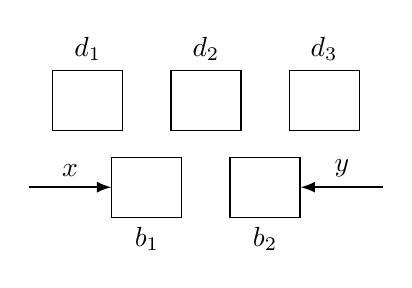
\begin{tikzpicture}[xscale=1.5]
      \node[dsnode, label={north:$d_1$}] (d1) at (1, 1.1) {};
      \node[dsnode, label={north:$d_2$}] (d2) at (2, 1.1) {};
      \node[dsnode, label={north:$d_3$}] (d3) at (3, 1.1) {};
      \node[replica, label={south:$b_1$}] (b1) at (1.5, 0) {};
      \node[replica, label={south:$b_2$}] (b2) at (2.5, 0) {};

      \draw[com] (0.5, 0) to node[above] {$x$} (b1);
      \draw[com] (3.5, 0) to node[above] {$y$} (b2);
    \end{tikzpicture}
    \caption{}\figlabel{SimpleBPaxosExample1}
  \end{subfigure}%
  \begin{subfigure}[b]{0.3\textwidth}
    \centering
    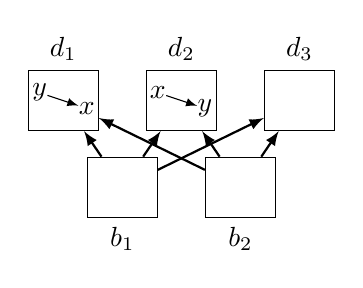
\begin{tikzpicture}[xscale=1.5]
      \node[dsnode, label={north:$d_1$}] (d1) at (1, 1.1) {};
      \node[dsnode, label={north:$d_2$}] (d2) at (2, 1.1) {};
      \node[dsnode, label={north:$d_3$}] (d3) at (3, 1.1) {};
      \node[replica, label={south:$b_1$}] (b1) at (1.5, 0) {};
      \node[replica, label={south:$b_2$}] (b2) at (2.5, 0) {};

      \draw[com] (b1) to (d1);
      \draw[com] (b1) to (d2);
      \draw[com] (b1) to (d3);
      \draw[com] (b2) to (d1);
      \draw[com] (b2) to (d2);
      \draw[com] (b2) to (d3);

      \node[cmd] (d1x) at (0.8, 1.2) {$y$};
      \node[cmd] (d1y) at (1.2, 1.0) {$x$};
      \node[cmd] (d2y) at (1.8, 1.2) {$x$};
      \node[cmd] (d2x) at (2.2, 1.0) {$y$};
      \draw[dep] (d1x) to (d1y);
      \draw[dep] (d2y) to (d2x);
    \end{tikzpicture}
    \caption{}\figlabel{SimpleBPaxosExample2}
  \end{subfigure}%
  \begin{subfigure}[b]{0.3\textwidth}
    \centering
    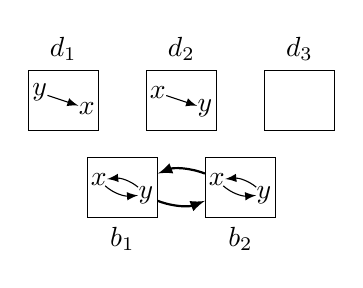
\begin{tikzpicture}[xscale=1.5]
      \node[dsnode, label={north:$d_1$}] (d1) at (1, 1.1) {};
      \node[dsnode, label={north:$d_2$}] (d2) at (2, 1.1) {};
      \node[dsnode, label={north:$d_3$}] (d3) at (3, 1.1) {};
      \node[replica, label={south:$b_1$}] (b1) at (1.5, 0) {};
      \node[replica, label={south:$b_2$}] (b2) at (2.5, 0) {};

      \draw[com, bend right] (b1) to (b2);
      \draw[com, bend right] (b2) to (b1);

      \node[cmd] (d1x) at (0.8, 1.2) {$y$};
      \node[cmd] (d1y) at (1.2, 1.0) {$x$};
      \node[cmd] (d2y) at (1.8, 1.2) {$x$};
      \node[cmd] (d2x) at (2.2, 1.0) {$y$};
      \draw[dep] (d1x) to (d1y);
      \draw[dep] (d2y) to (d2x);

      \node[cmd] (b1x) at (1.3, 0.1) {$x$};
      \node[cmd] (b1y) at (1.7, -0.1) {$y$};
      \node[cmd] (b2x) at (2.3, 0.1) {$x$};
      \node[cmd] (b2y) at (2.7, -0.1) {$y$};
      \draw[dep, bend right] (b1x) to (b1y);
      \draw[dep, bend right] (b1y) to (b1x);
      \draw[dep, bend right] (b2x) to (b2y);
      \draw[dep, bend right] (b2y) to (b2x);
    \end{tikzpicture}
    \caption{}\figlabel{SimpleBPaxosExample3}
  \end{subfigure}

  \caption{Example Simple BPaxos execution}\figlabel{SimpleBPaxosExample}
\end{figure}
